\documentclass[11pt]{article}
\usepackage{amssymb}
\usepackage{amsmath}
\usepackage{amsthm}
\usepackage{fullpage}
\usepackage{hyperref}
\usepackage{multicol}
\usepackage{svg}
\usepackage[h]{esvect}
\usepackage{graphicx}
\usepackage{tikz}
% \usepackage{pgfplots}
\usetikzlibrary{arrows.meta}
\usepackage{gensymb}
\setlength{\parskip}{1ex}
\setlength{\parindent}{0pt}
\def\N {{\mathbb N}}
\def\Z {{\mathbb Z}}
\def\R {{\mathbb R}}
\def\comp {{\mathrm{comp}}}
\def\proj {{\mathrm{proj}}}
\def\Grad {\mathrm{grad\,}}
\def\Div {\mathrm{div\,}}
\def\Curl {\mathrm{curl\,}}
\newcommand{\partialderiv}[2] {\frac{\partial #1}{\partial #2}}
\newcommand{\Implies}{\mbox{ IMPLIES }}
\newcommand{\Or}{\mbox{ OR }}
\renewcommand{\And}{\mbox{ AND }}
\newcommand{\Not}{\mbox{NOT}}
\newcommand{\Iff}{\mbox{ IFF }}
\newcommand{\True}{\mbox{T}}
\newcommand{\False}{\mbox{F}}
\newcommand{\norm}[1]{\lVert #1 \rVert}
\usepackage{listings}
\usepackage{xcolor}

\definecolor{codegreen}{HTML}{237e02}
\definecolor{codegray}{rgb}{0.5,0.5,0.5}
\definecolor{codepurple}{HTML}{8F4673}
\definecolor{codebrown}{HTML}{ce9178}
\definecolor{codecyan}{HTML}{098658}
\lstdefinestyle{pythonstyle}{
    commentstyle=\color{codegreen},
    keywordstyle=\color{codepurple},
    numberstyle=\tiny\color{codegray},
    stringstyle=\color{codebrown},
    basicstyle=\ttfamily\small,
    breakatwhitespace=false,         
    breaklines=true,                 
    captionpos=b,                    
    keepspaces=true,                 
    numbers=none,                    
    numbersep=5pt,                  
    showspaces=false,                
    showstringspaces=false,
    showtabs=false,                  
    tabsize=2
}

\lstset{style=pythonstyle}

\newtheorem{theorem}{Theorem}[section]
\newtheorem{corollary}{Corollary}[theorem]
\newtheorem{lemma}[theorem]{Lemma}
\newtheorem{definition}[theorem]{Definition}
\newcounter{example}[section]
\newenvironment{example}[1][]{\refstepcounter{example}\par\medskip
   \noindent \textbf{Example~\theexample. #1} \rmfamily}{\par \begin{flushright} \textbf{End of Example~\theexample} \end{flushright}}

\begin{document}
\begin{center}

{\bf \Large \bf MATH209 Summer 2021 Tets 2.2}\\
{\bf \large Kevin Gao}
\end{center}

\begin{enumerate}
    \item Question 1
    $$
    T(\rho,\theta,\phi) = (\rho \sin\phi \cos\theta, \rho \sin\phi \sin\theta, \rho \cos\phi)
    $$
    By definition of the Jacobian,
    $$
    \begin{aligned}
    J(\rho, \theta, \phi) &= \begin{vmatrix}
    \displaystyle \partialderiv{x}{\rho} & \displaystyle \partialderiv{x}{\theta} & \displaystyle \partialderiv{x}{\phi} \\
    \hfill \\
    \displaystyle \partialderiv{y}{\rho} & \displaystyle \partialderiv{y}{\theta} & \displaystyle \partialderiv{y}{\phi} \\
    \hfill \\
    \displaystyle \partialderiv{z}{\rho} & \displaystyle \partialderiv{z}{\theta} & \displaystyle \partialderiv{z}{\phi}
    \end{vmatrix} \\
    &= \partialderiv{x}{\rho} \begin{vmatrix}
    \partialderiv{y}{\theta} & \partialderiv{y}{\phi} \\
    \partialderiv{z}{\theta} & \partialderiv{z}{\phi}
    \end{vmatrix} - 
    \partialderiv{x}{\theta} \begin{vmatrix}
    \partialderiv{y}{\rho} & \partialderiv{y}{\phi} \\
    \partialderiv{z}{\rho} & \partialderiv{z}{\phi}
    \end{vmatrix} + 
    \partialderiv{x}{\phi} \begin{vmatrix}
    \partialderiv{y}{\rho} & \partialderiv{y}{\theta} \\
    \partialderiv{z}{\rho} & \partialderiv{z}{\theta}
    \end{vmatrix}
    \end{aligned}
    $$
    And since
    $$
    \partialderiv{x}{\rho} = \sin\phi\cos\theta \qquad
    \partialderiv{x}{\theta} = -\rho \sin\phi \sin\theta \qquad \partialderiv{x}{\phi} = \rho\cos\phi\cos\theta
    $$
    $$
    \partialderiv{y}{\rho} = \sin\phi\sin\theta \qquad
    \partialderiv{y}{\theta} = \rho \sin\phi \cos\theta \qquad \partialderiv{y}{\phi} = \rho\cos\phi\sin\theta
    $$
    $$
    \partialderiv{z}{\rho} = \cos\phi \qquad
    \partialderiv{z}{\theta} = 0 \qquad
    \partialderiv{z}{\phi} = -\rho\sin\phi
    $$
    We can evaluate the Jacobian as
    $$
    \begin{aligned}
    J(\rho,\theta,\phi) &= -\rho \sin^3\cos^2\theta - \rho^2\sin^2\phi\sin^2\theta - \rho^2 \sin\phi \cos^2\phi \cos^2\theta \\
    &= -\rho^2 (\sin\phi\sin^2\phi + \sin\phi\sin^2\theta + \sin\phi\cos^2\phi\cos^2\theta) \\
    &= -\rho^2\sin\phi(\sin^2\phi\cos^2\theta + \sin^2\theta + \cos^2\phi\cos^2\theta) \\
    &= -\rho^2\sin\phi (\sin^2\theta + \cos^2\theta ( \sin^2\phi + \cos^2\phi)) \\
    &= -\phi^2\sin\phi (\sin^2 \theta + \cos^2 \theta) \\
    &= -\phi^2\sin\phi
    \end{aligned}
    $$
    We take the absolute value of the result, which gives us the final answer
    $$
    J(\rho,\theta,\phi) = \rho^2\sin\phi
    $$
    
    \item Question 2
    \begin{enumerate}
        \item We find a general expression of $\Curl \vv F$
        $$
        \begin{aligned}
        \Curl \vv F &= \left( \partialderiv{R}{y} - \partial{Q}{z} \right) \hat{i} + \left( \partialderiv{P}{z} - \partial{R}{x} \right) \hat{j} + \left( \partialderiv{Q}{x} - \partial{P}{y} \right) \hat{k} \\
        &= (0, (a-4)z^2, (a-4)x)
        \end{aligned}
        $$
        Then, when $a=4$, $\Curl \vv F = 0$ and $\vv F$ is irrotational.
        
        \item Similarly, we find a general expression of $\Div \vv F$
        $$
        \begin{aligned}
        \Div \vv F &= \partialderiv{P}{x} + \partialderiv{Q}{y} + \partialderiv{R}{z} \\
        &= a^2 - a -6
        \end{aligned}
        $$
        Then, when $a=-2$ or $a=3$, $\Div \vv F = 0$ and $\vv F$ is soleinoidal.
    \end{enumerate}
    
    \item Question 3
    \begin{enumerate}
        \item 
        $$
        \int_C (x^2y^3 - \sqrt{x})dy
        $$
        where $C$ is the arc of the curve $y=\sqrt{x}$ from $(1,1)$ to $(4,2)$.
        
        We can parameterize the curve as
        $$
        x(t) = t \qquad y(t) = \sqrt{t} \qquad 1 \leq t \leq 4
        $$
        
        Then, we can write the line integral as
        $$
        \begin{aligned}
            \int_C f(x,y) dy &= \int_1^4 f(x(t),y(t)) y'(t) dt \\
            &= \int_1^4 f(t,\sqrt{t}) \cdot \frac{1}{2}t^{-1/2} dt \\
            &= \int_1^4 (\sqrt{t}(t^3-1)) \cdot \frac{1}{2}t^{-1/2} dt \\
            &= \frac{1}{2} \int_1^4 (t^3-1) dt \\
            &= 30.375
        \end{aligned}
        $$
        
        \item
        $$
        \int_C (2x+9z) ds
        $$
        where $C:\; x=t, y=t^2, z=t^3,\; 0 \leq t \leq 1$.
        
        The line integral can be evaluated as
        $$
        \begin{aligned}
            \int_C f(x,y,z) ds &= \int_0^1 f(x(t),y(t),z(t)) \sqrt{\frac{dx}{dt}^2 + \frac{dy}{dt}^2 + \frac{dz}{dt}^2} dt \\
            &= \int_0^1 (2t+9t^3) \sqrt{1+4t^2+9t^4} dt \\
            &= 8.56
        \end{aligned}
        $$
    \end{enumerate}
    
    \item Question 4
    $$
    \vv F(x,y) = (P(x,y), Q(x,y))
    $$
    We first check whether or not $\partialderiv{P}{y} = \partialderiv{Q}{x}$.
    $$
    \partialderiv{P}{y} = e^{xy} + 6xy^2 + xye^{xy} \qquad \partialderiv{Q}{x} = e^{xy} + 6xy^2 + xye^{xy}
    $$
    The vector field is conservative.
    
    Then, to find the potential function, let 
    $$
    f(x,y) = \int P\, dx + \phi(y) = e^{xy}+\sin(x)+x^2y^3-6x^3 + \phi(y)
    $$
    Find $\partialderiv{f}{y}$
    $$
    \partialderiv{f}{y} = xe^{xy} + 3x^2y^2 + \phi'(y)
    $$
    Set $\partialderiv{f}{y} = xe^{xy} + 3x^2y^2 + \phi'(y) = Q(x,y)$ and solve for $\phi'(y)$.
    $$
    \phi'(y) = -\sec^2 y + 5e^{5y} \qquad \phi(y) = \int \phi'(y) dy = e^{5y}-\tan y + C
    $$
    Hence the potential function $f$ is
    $$
    f(x,y) = e^{xy}+\sin(x)+x^2y^3-6x^3 + e^{5y}-\tan y + C
    $$
    
    \item Question 5
    \begin{figure}[h]
        \centering
        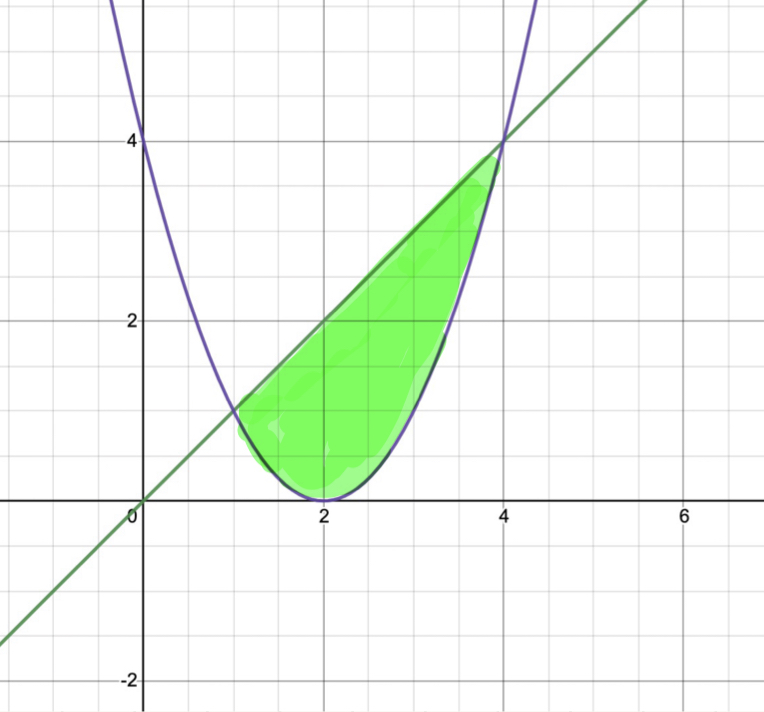
\includegraphics[width=0.45\linewidth]{figures/test221.PNG}
        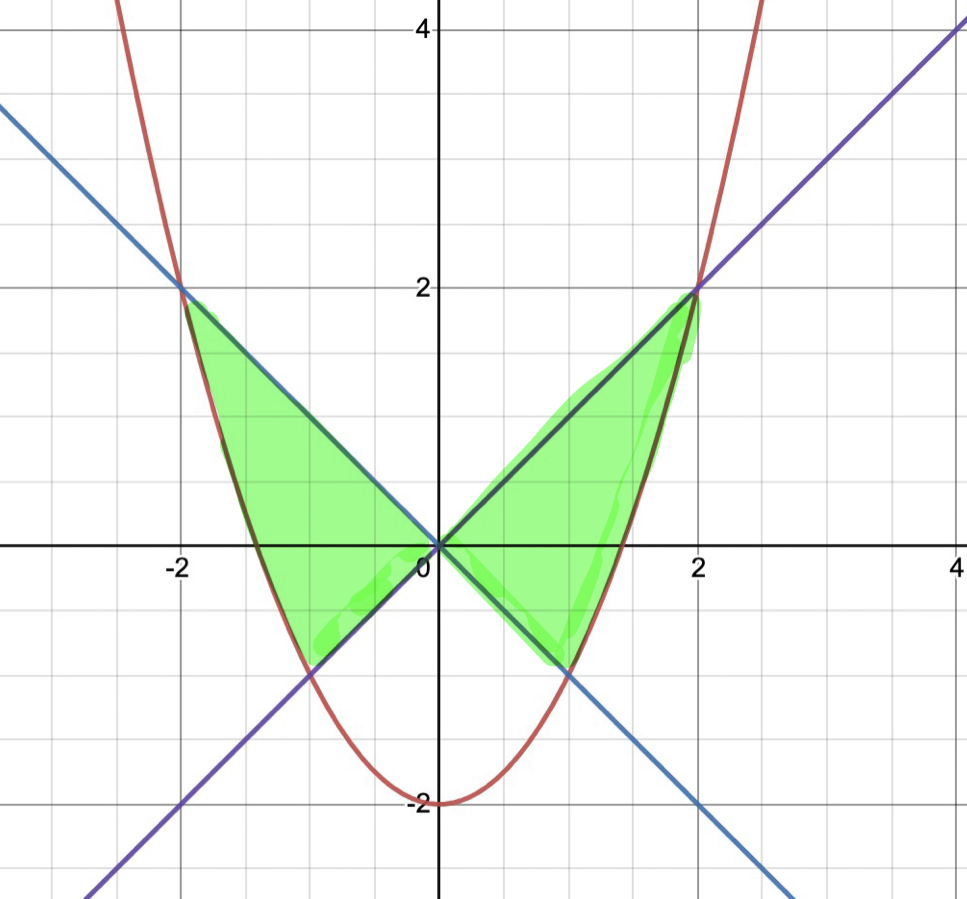
\includegraphics[width=0.45\linewidth]{figures/test222.PNG}
    \end{figure}
    \begin{enumerate}
        \item 
        $$
        \int_{1}^{4}\int_{\left(y-2\right)^{2}}^{y}dxdy
        $$
        
        \item
        $$
        \int_{-2}^{0}\int_{\left(y^{2}-2\right)}^{-y}f(x,y)dxdy\ +\int_{0}^{2}\int_{\left(y^{2}-2\right)}^{y}f(x,y)dxdy\ 
        $$
    \end{enumerate}
    
    \item Question 6
    \begin{enumerate}
        \item The area of integration is
        $$
        \{ (x,y) \mid 0 \leq x \leq 2,\; 1.5x+1 \leq y \leq -2.5+9 \}
        $$
        Then,
        $$
        \begin{aligned}
        A(S) &= \iint_D \sqrt{f_x(x,y)^2 + f_y(x,y)^2 + 1} dA \\
        &= \int_0^2 \int_{1.5x+1}^{-2.5+9} \sqrt{f_x(x,y)^2 + f_y(x,y)^2 + 1} dy \, dx \\
        &= \int_0^2 \int_{1.5x+1}^{-2.5+9} \sqrt{\frac{1}{4}x^2 + \frac{1}{4} + 1} \\
        &= \int_0^2 \int_{1.5x+1}^{-2.5+9} = \frac{1}{2}\sqrt{x^2+5} \\
        &= \int_0^2 (4-2x) \sqrt{x^2+5} \\
        &\approx 9.5
        \end{aligned}
        $$
        
        \item The paraboloid does not intersect with the plane as
        $$
        2 = 1 - x^2 - y^2
        $$
        does not have a real solution. Hence, the surface area is 0.
        
        \item Again, the surface area can be expressed as
        $$
        \begin{aligned}
        A(S) &= \iint_D \sqrt{f_x(x,y)^2 + f_y(x,y)^2 + 1)} dA \\
        &= \iint_D \sqrt{1+4x^2+4y^2} dA \\
        &= \iint_D \sqrt{1+4(x^2+y^2)} dA
        \end{aligned}
        $$
        Transform this double integral into polar coordinate
        $$
        \begin{aligned}
        A(S) &= \iint_D r \sqrt{1+4r^2} dr d\theta
        \end{aligned}
        $$
        Since we are after the region between the cylinders $x^2+y^2=1$ and $x^2+y^2=4$, we can define the limits of integration
        $$
        \begin{aligned}
        A(S) &= \iint_D r \sqrt{1+4r^2} dr d\theta \\
        &= \int_0^{2\pi}\int_1^4 r \sqrt{1+4r^2} dr d\theta \\
        &\approx 30.85
        \end{aligned}
        $$
    \end{enumerate}
    
    \item Question 7
    \begin{enumerate}
        \item We first define $C$ as the following line segments
        $$
        \begin{aligned}
        C_1&:\; (1,1) + (2,-6)t \qquad 0 \leq t \leq 1 \\
        C_2&:\; (3,-5) + (-5,3)t \qquad 0 \leq t \leq 1 \\
        C_3&:\; (-2,-2) + (1,5)t \qquad 0 \leq t \leq 1
        \end{aligned}
        $$
        Since $\vv F$ is a conservative vector field, it has a potential function $f$.
        $$
        f(x,y) = \int 3x^2 + 2xy \; dx + \phi(y)
        $$
        where $\partialderiv{f}{y} = 3y^2+x^2$. Hence, $\phi(y) = y^3$, and
        $$
        f(x,y) = x^3+x^2y+y^3
        $$
        Then, by the Fundemental Theorem for Line Integral,
        $$
        \begin{aligned}
        \int_C \vv F \cdot d\vv r &= \int_{C_1} \vv F \cdot d\vv r + \int_{C_2} \vv F \cdot d\vv r + \int_{C_3} \vv F \cdot d\vv r \\
        &= (f(\vv r_1(b))-f(\vv r_1(a))) + (f(\vv r_2(b))-f(\vv r_2(a))) + (f(\vv r_3(b))-f(\vv r_3(a))) \\
        &= (f(3,-5)-f(1,1)) + (f(-2,-2)-f(3,-5)) + (f(-1,3)-f(-2,-2)) \\
        &= 26
        \end{aligned}
        $$
        
        \item Since $\vv F$ is conservative, its line integral is path independence.
        
        And since we are taking the line integral with respect to an ellipse (closed curve),
        $$
        \oint_C \vv F \cdot d\vv r = 0
        $$
    \end{enumerate}
    
    \item Question 8
    
    The region of integration is sketched in the following diagram.
    \begin{figure}[h]
        \centering
        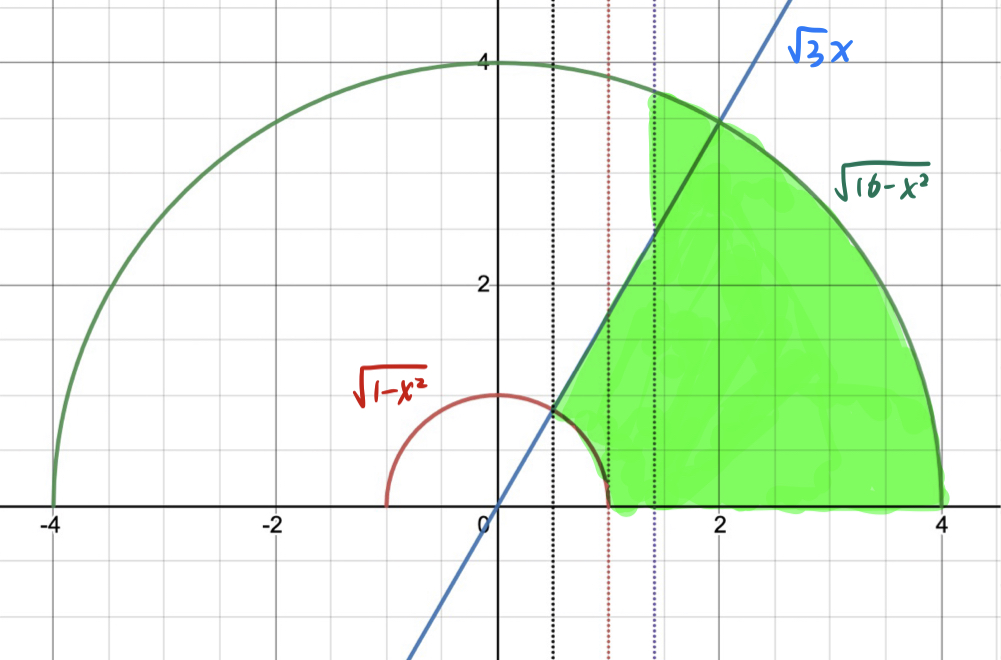
\includegraphics[width=0.45\linewidth]{figures/test223.PNG}
    \end{figure}
    The region that is enclosed inside the two half circle can be evaluated using polar coordinates, and the remaining region still needs to be calculated using iterated integral.
    $$
    \begin{aligned}
    \int_{0}^{\frac{\pi}{3}}\int_{1}^{4}rr^{2}\sin\left(\theta\right)\cos\left(\theta\right)\ drd\theta + \int_{\sqrt{2}}^{2}\int_{\sqrt{3}x}^{\sqrt{16-x^{2}}}xydydx = 23.90625 + 2 = 25.90625
    \end{aligned}
    $$
    
    \item Question 9
    \begin{enumerate}
        \item Let $x=1/2(u+v)$ and $y=1/2(u-v)$ with a Jacobian of $1/2$.
        
        This also implies that
        $$
        u = x+y \qquad v = x-y
        $$
        Then, the region of integration becomes
        $$
        \{ (u,v) \mid 0 \leq u \leq 3,\; 0 \leq v \leq 2 \}
        $$
        We can evaluate the integral as
        $$
        \frac{1}{2} \iint_S ue^{uv} dA = \frac{1}{2}\int_0^2 \int_0^3 ue^{uv} dudv = 99.1
        $$
        
        \item Let $x=u+v$ and $v=2u-v$ with a Jacobian of $1/3$.
        
        Then, the region of integration becomes
        $$
        \{ (u,v) \mid 0 \leq u \leq 1/3,\; -1 \leq v \leq 2/3 \}
        $$
        We can evaluate the integral as
        $$
        \int_{0}^{1}\int_{0}^{\frac{1}{3}}\sqrt{3u}9v^{2}dudv = \frac{2}{9}
        $$
    \end{enumerate}
    
    \item Question 10
    \begin{enumerate}
        \item 
        $$
        \begin{aligned}
        \int_C \vv F \cdot d\vv r &= \int_0^1 \vv F(\vv r(t)) \cdot \vv r'(t) dt \\
        &= \int_0^1 \vv F(11t^4, t^3) \cdot (44t^3, 3t^2) dt \\
        &= \int_0^1 (11t^7, 3t^9) \cdot (44t^3, 3t^2) dt \\
        &= \int_0^1 484t^{10} + 9t^{11} \, dt \\
        &= 179/4
        \end{aligned}
        $$
        
        \item
        
        Using Green's Theorem. Since the curve is negatively-oriented, we need to change the sign.
        $$
        \begin{aligned}
        \oint_C \vv F \cdot d\vv r &= -\oint_C \left( \partialderiv{Q}{x} - \partialderiv{P}{y} \right) dA \\
        &= -\oint y \, dA
        \end{aligned}
        $$
        Convert to polar coordinate,
        $$
        \int_{0}^{2\pi} \int_0^3 r\cdot r^2 \sin\theta \, drd\theta = 0
        $$
    \end{enumerate}
    
    \item Question 11
    \begin{enumerate}
        \item 
        $$
        \int_0^4 \int_{\sqrt{x}}^2 \frac{1}{y^3+1} = \int_0^2 \int_0^{x^2} \frac{1}{y^3+1} = \frac{2}{3} \ln 3
        $$
        
        \item Transform into polar coordinate
        $$
        \int_{-3}^3 \int_0^{\sqrt{9-x^2}} \sin(x^2+y^2) dydx = \int_0^\pi \int_0^3 r\sin(r^2) dr d\theta = \frac{\pi}{2}(1-\cos9)
        $$
    \end{enumerate}
\end{enumerate} 

\end{document}